\section{Halbleiter}

\subsubsection{Leitfähigkeit / elektrischer Widerstand}

\begin{minipage}[t]{0.48\columnwidth}
	\myul{\textbf{Leitfähigkeit $\bm{\kappa}$}}
	$$ \boxed{ \kappa = \frac{1}{\rho} = n \cdot q \cdot \mu } $$
\end{minipage}
\hfill
\begin{minipage}[t]{0.48\columnwidth}
	\myul{\textbf{(Leiter-)Widerstand}}
	$$ \boxed{ R = \frac{\rho \cdot l}{A} = \frac{l}{ \kappa \cdot A} } $$
\end{minipage}

\vspace{0.2cm}

\myul{\textbf{Temperaturabhängigkeit (1. Näherung linear)}}
$$ \boxed{ \rho(T) = \rho(T_0) \cdot (1  + \alpha(T - T_0)) } $$


\begin{tabular}{clc}
	$n$ 						& Ladungsträgerdichte 									& 												\\
	$q$ 						& Elementarladung $q = 1.6 \cdot 10^{-19} \, \coulomb$ 	& $[q] = \coulomb$								\\
	$l$ 						& Läge des Leiters 										& $[l] = \meter$ 								\\
	$A$ 						& Querschnittsfläche des Leiters 						& $[A] = \meter^2$ 								\\
	$\mu$ 						& Beweglichkeit der Ladungsträger 						& 												\\
	$\alpha$ 					& Temperaturkoeffizient 								& $[\alpha] = \frac{1}{\kelvin}$ 				\\
	$\kappa = \frac{1}{\rho}$ 	& Spez. Leitfähigkeit bzw. spez. Widerstand 			& $[\kappa] = \frac{\meter}{\ohm \cdot \milli \meter}$
\end{tabular}


\subsubsection{Elektrische Eigenschaften von (Halb-)Leitern / Isolatoren}

\begin{tabular}{ll}
	Leiter 		& \textbf{positiver} Temperaturkoeffizent $\alpha$ 									\\
				& Leitfähigkeit Metalle: $10^6 \ldots 10^8 \, \frac{\siemens}{\meter}$ (2 Dekaden) 	\\
	Halbleiter 	& \textbf{negativer} Temperaturkoeffizent $\alpha$ 									\\
				& \textbf{Dotierung} Verändert Leitfähigkeit (10 Dekaden) 							\\
	Isolatoren 	& Kein Temperaturkoeffizent $\alpha$ 
\end{tabular}


\subsection{Dotierung von Halbleitern}

Unter \textbf{Dotierung} versteht man das Einbringen von Fremdatomen ins Kristallgitter des Halbleiters (z.B. von Silizium)

\begin{center}
	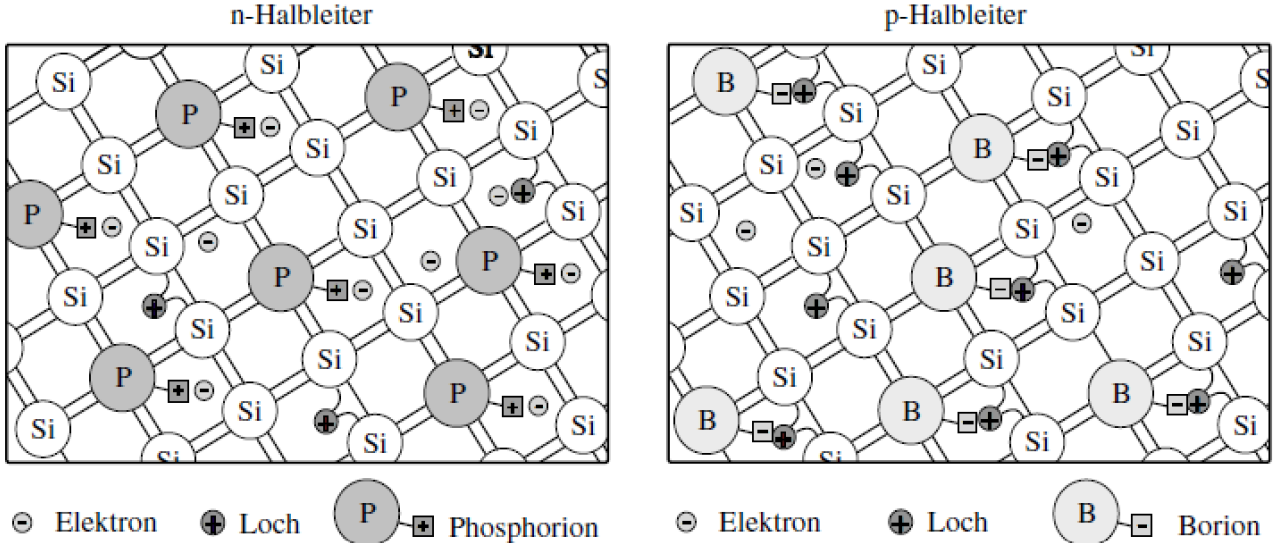
\includegraphics[width=0.75\columnwidth]{images/dotierung.png}
\end{center}


\begin{tabular}{ll}
	\textbf{n-Dotierung} 	& Zufügen von Atomen mit 5 Elektronen 		\\
							& \textrightarrow\ Elektronen-Überschuss 	\\
	\textbf{p-Dotierung} 	& Zufügen von Atomen mit 3 Elektronen 		\\
							& \textrightarrow\ Löcher-Überschuss
\end{tabular}

\vspace{0.2cm}

\textrightarrow\ p-Dotierung ist immer schlechter (geringere Leitfähigkeit), da Elektronen fehlen


\subsection{pn-Übergang}

\begin{tabular}{| ll | ll |}
	\hline
	P-Anschluss: 	& Anode 	& RLZ: 	& Raumladungszone	\\
	N-Anschluss: 	& Kathode 	& \el 	& Elektron 			\\
	\hline
\end{tabular}


\subsubsection{pn-Übergang ohne äussere Spannung}

\begin{minipage}[c]{0.3\columnwidth}
	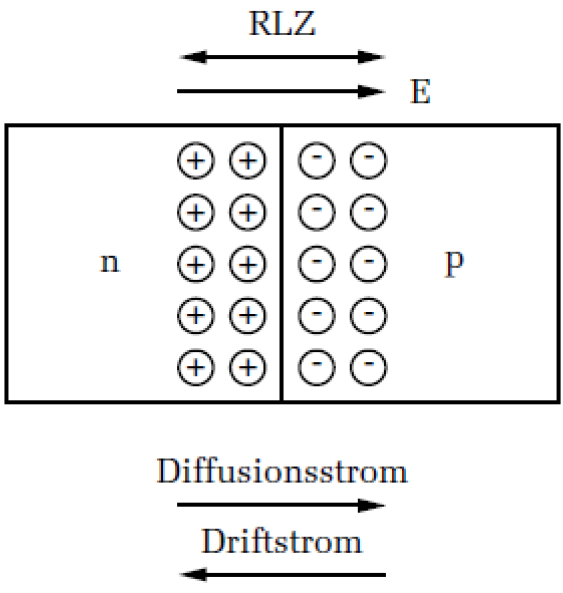
\includegraphics[width=\columnwidth]{images/pn-uebergang.png}
\end{minipage}
\hfill
\begin{minipage}[c]{0.65\columnwidth}
	\textbf{Diffusionsstrom: Dichte-Ausgleich} \\
	\el diffundieren in p-Zone, Löcher in n-Zone

	\vspace{0.2cm}

	\textbf{Driftstrom: Durch elektrisches Feld} \\
	\el von positiver Spannung in n-Zone angezogen \\
	\textrightarrow\ Es entsteht ein Gleichgewicht!

	\vspace{0.2cm}

	Zwischen p- und n-Bereich entsteht isolierende \textbf{RLZ}
\end{minipage}

